\subsection{Resultados Punto 6: Envolvente Compleja en el Tiempo}
El análisis temporal de la señal modulada se enfocó en su envolvente compleja, la cual caracteriza completamente a la señal pasabanda sin necesidad de simular la alta frecuencia de la portadora.

En la Figura \ref{fig:envolvente_clase} se presentan las componentes en-fase (línea azul) y en cuadratura (línea roja) de la señal 8-PSK procesadas por el filtro interpolador, en un escenario libre de ruido. Es evidente cómo el filtro mantiene los niveles de voltaje y genera transiciones escalonadas bien definidas entre los distintos estados de fase. Esta periodicidad visualizada es característica de una transmisión secuencial de la fuente de datos y demuestra la correcta generación de los 8 niveles de amplitud independientes en los ejes real e imaginario.

\begin{figure}[htbp]
    \centering
    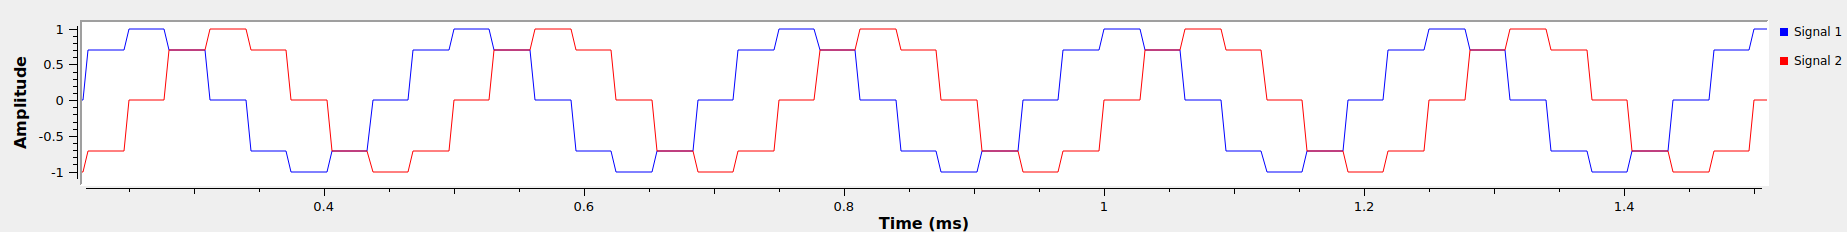
\includegraphics[width=0.9\linewidth]{imagenes/envolvente_compleja_punto6.png}
    \caption{Señal de envolvente compleja en el dominio del tiempo (canal ideal).}
    \label{fig:envolvente_clase}
\end{figure}

Finalmente, la Figura \ref{fig:envolvente_ruido} expone el comportamiento de la misma envolvente compleja al ser afectada por el canal AWGN. Se nota una perturbación constante en la amplitud de las componentes ortogonales. Teóricamente, esta suma de componentes aleatorias se traduce en una dispersión de los puntos en el diagrama de constelación del receptor, lo que aumenta la probabilidad de que un símbolo invada la región de decisión adyacente, incrementando la tasa de error de símbolo (SER) del sistema de comunicaciones.

\begin{figure}[H]
    \centering
    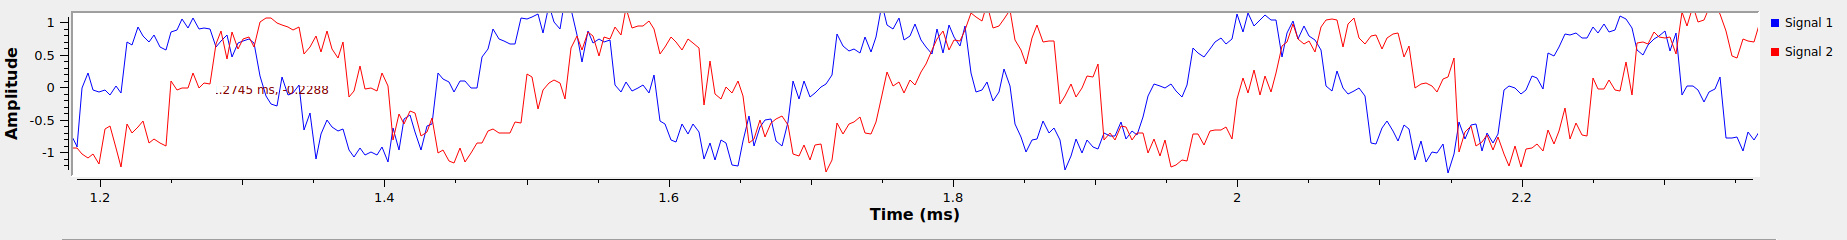
\includegraphics[width=0.9\linewidth]{imagenes/envolvente_tiempo.png}
    \caption{Señal de envolvente compleja afectada por el canal AWGN.}
    \label{fig:envolvente_ruido}
\end{figure}